\stopallthesefloats
\subsection{WUPPAAL}
\begin{figure}[hbt]
\begin{center}
\centering
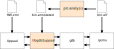
\includegraphics[width=0.7\textwidth]{\chapterdirectory/figure/analysis/wuppaal.pdf}
\end{center}
\caption{Overview of WUPPAAL's components (taken from \cite{wuppaal})}%
\label{fig:formal_analysis:wuppaal}
\end{figure}

\cite{wuppaal} describes WUPPAAL, another approach to using UPPAAL in order to
compute the WCET of a program running on a single-core processor. The main
novelty of \cite{wuppaal} is that it combines simulated execution with the
model checking. Indeed, as can be seen in
Figure~\ref{fig:formal_analysis:wuppaal}, it allows UPPAAL to interact with
\textit{qemu} (an architecture simulation tool) through \textit{gdb} (a
debugging tool) and \textit{libgdbuppaal} (a library of their own making). The
\textit{pre-analysis} step shown in the figure corresponds to the annotation of
a binary program with information in order to help the extraction its
\textit{Control Flow Graph}. This approach aims at improving the memory usage
of model checking, as well as making the approach fit other architectures very
easily (by just changing qemu parameters).

These annotations allow the generation of an over-approximation of all valid
program runs from the CFG. This has some surprising results, such as
deterministic programs having multiple separate runs because the
over-approximation does not consider actual values for any computation
involving input parameters. Instead, all outcomes are considered, even if some
sequences of outcomes cannot follow one another (e.g.~the exact same test
failing once, then succeeding). For such runs to be finite, loops cannot be
controlled by input parameters (i.e.~all loops have a known amount of
iterations).

\begin{figure}[hbt]
\begin{center}
\centering
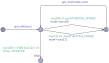
\includegraphics[width=0.7\textwidth]{\chapterdirectory/figure/analysis/wuppaal_automaton.pdf}
\end{center}
\caption{Automaton interacting with \textit{libgdb2uppaal} (taken from
\cite{wuppaal})}%
\label{fig:formal_analysis:wuppaal_automaton}
\end{figure}

UPPAAL is used to perform queries among all possible execution paths. However,
in WUPPAAL, the automaton corresponding to the program is not a purely UPPAAL
one. Figure~\ref{fig:formal_analysis:wuppaal_automaton} shows the automaton in
question.  It does not store full program states, and instead only keeps an
identifier and the annotations for current instruction. The function calls seen
on the automaton actually trigger another component from
Figure~\ref{fig:formal_analysis:wuppaal}: \textit{libgdbuppaal}. This component
is where program states are stored. \textit{libgdbuppaal} uses \textit{qemu} to
compute the program state resulting from the application of the instruction, as
well as all possible next execution nodes. The program state inserted back in
UPPAAL indicates whether the instruction was found in the cache and how long its
execution stage lasts.

UPPAAL is then involved in the computation of the WCET for these annotated
traces. Indeed, it models the pipelines, with one automaton per stage, as well
as a main memory automaton and an instruction cache one (see
Figure~\ref{fig:formal_analysis:wuppaal_cache}), to model their access times.
Since the information about whether the instruction cache contains the
instruction or not is already in the annotated execution trace, these last two
automata are kept very simple.

\begin{figure}[hbt]
\begin{center}
\centering
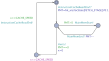
\includegraphics[width=0.7\textwidth]{\chapterdirectory/figure/analysis/wuppaal_cache.pdf}
\end{center}
\caption{WUPPAAL Instruction Cache Automaton (taken from
\cite{wuppaal})}%
\label{fig:formal_analysis:wuppaal_cache}
\end{figure}

Figure~\ref{fig:formal_analysis:wuppaal_cache} shows the automaton
corresponding to an instruction cache in WUPPAAL. The initial state is the top
one. Upon receiving a request for reading on \textbf{InstructionCacheReadStart}
(considering the rest of the variables, writing likely uses the same channel),
the automaton checks if the information is already in the cache. If not it
performs as many synchronizations with the main memory automaton as is needed
(indicated by \textit{PMT}), then waits a time corresponding to that of a
cache access before using \textbf{InstructionCacheReadEnd} to signal the
completion of the request.

\stopallthesefloats
